\section{Scalable to Real-world Crypto Systems}

In the section, we articulate several challenges and existing problems
in quantifying the side-channel vulnerability leakages. We describe the
challenges and then briefly present the corresponding solution.

\subsection{Challenge I: Information Leakage Definition}

Existing static-based side-channel quantification works~\cite{182946} define information leakage
as the mutual information or the maximal leakage. These definitions provide a strong security guarantee
when trying to prove a program is secure enough if their methods calculate the program 
leaks zero bits of information.


\begin{figure}[h!]
\centering
    % \vspace{-5mm}
\begin{lstlisting}[xleftmargin=.03\textwidth,xrightmargin=.01\textwidth]
unsigned char key = input();
// key = [0 ... 255]
if(key = 128)
    A(); // branch 1
else if (key < 64)
    B(); // branch 2
else if (key < 128)
    C(); // branch 3
else
    D(); // branch 4
\end{lstlisting}
\caption{Side-channel leakage}
\label{code::entropy}
    % \vspace{-5mm}
\end{figure}

However, the above definition is less useful to justify the sensitive level of leakage sites. 
Considering the example code~\ref{code::entropy}, if an attacker knows the
code executes branch A by some observations, the attacker can know the key actually equals to 128. 
Suppose it is a dummy password checker, in which case the attacker can fully retrieve the password.
Therefore, the total information leakage should be 8 bits, which equals to the size
of unsigned char. 
According to the mutual definition, however, the leakage will be 1.7 bits. \fixme{use footnote or list the calculation process}. The maximal information
leakage is 2 bits. \fixme{the same with previous}. Both approaches fail to tell how 
much information is leaked during the execution precisely.

The problem with the existing methods is that they are static-based and the 
input values are neglected by the previous definition. 
They assume the attacker runs the program multiple times with many different sensitive 
information as the input. Both the mutual information and the max-leakage give an ``average" 
estimate of the information leakage. However, it isn't the typical scenario for an adversary to 
launch an side-channel attack. When a side-channel attack happens, the adversary wants 
to retrieve the sensitive information, in which case the sensitive information is fixed (e.g. AES keys). 
The adversary will run the attack over and over again and guess the value bit by bit. Like the 
previous example, the existing static method does not work well in those situations.

\begin{figure}
  \centering
   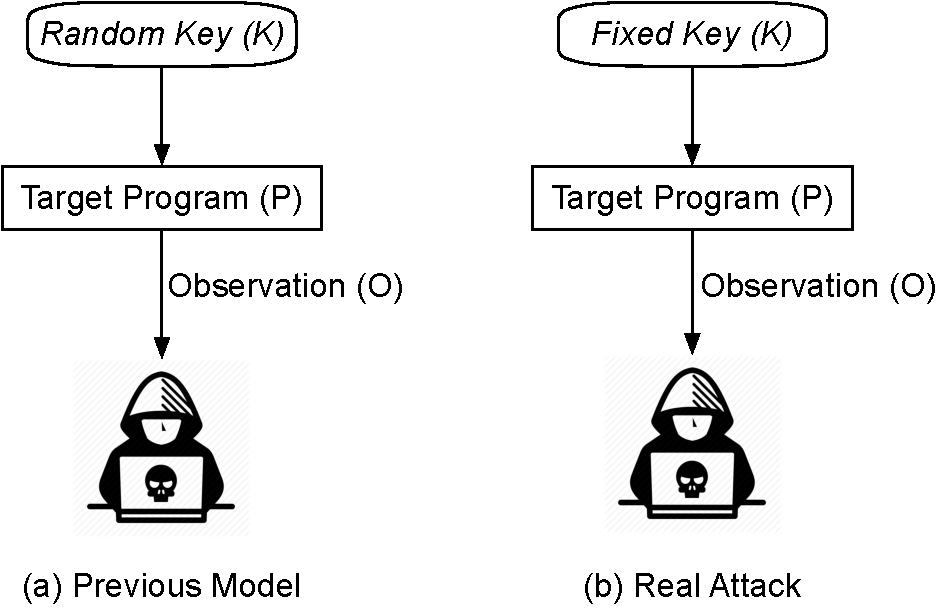
\includegraphics[width=.9\columnwidth]{./figures/RA.pdf}
   \caption{\fixme{some caption here}}
\end{figure}

\vspace*{6pt}
\textbf{Our Solution to Challenge I:}
In the project, we hope to give a very precise definition of information leakages. 
Suppose an attacker run the target program multiple times with one fixed input, we
want to know how much information he can infer by observing the memory access patterns.
We come to the simple slogan ~\cite{10.1007/978-3-642-00596-1_21} %% where the information
%% leakage equals:
%% \textbf{Initial uncertainty - remaining uncertainty}
that
\begin{align*}
 & \mathit{Information\ leakage} = \\
 & ~~~~~~ \mathit{Initial}\ \mathit{uncertainty} - \mathit{Remaining\ uncertainty}. 
\end{align*}


If an adversary has zero knowledge about the input before the attack. The initial uncertainty
equals to the size the input. As for the remaining uncertainty, we come to the original definition
of the information content.
We quantify the information leakage with the following definition. 

\newtheorem{mydef}{Definition}

\begin{mydef}
\label{def}
Given a program $P$ with the input set $K$, 
an adversary has the observation $o$ when the input $k{\in}K$. 
We denote it as
    $$P(k) = o.$$
The leakage $L_{P(k)=o}$ based on the oberservation is
    $$L_{P(k)=o} = \log_2{|K|} - \log_2{|K^o|}$$
    where
    $$K^o = \{k | k \in K \ \text{and} \ P(k) = o \}$$
\end{mydef}

With the new definition, if the attacker observes that the code~\ref{code::entropy} runs the branch 1, 
then the $K^{o^{1}} = \{128\}$. Therefore, the information leakage $L_{P(k)=o^{1}} = \log_2{256} - \log_2{1} = 8$
bits, which means the key is totally leaked. If the attacker observes the code runs other
branches, the leaked information is shown in the following table.

\begin{table}[h]
    \centering
    \resizebox{.7\columnwidth}{!}{
    \begin{tabular}{|c|c|c|c|c|}
    \hline
    Branch & 1 & 2  & 3  & 4   \\ \hline
    $K^o$   & 1 & 64 & 64 & 127 \\ \hline
    $L_{P(k)=o}$(bits)   & 8 & 2  & 2  & 1   \\ \hline
    \end{tabular}
    }
    \caption{The leaked information by the definition~\ref{def}}
\end{table}

With the same definition~\ref{def}, if the attacker observes that the code run branch 2, the information
leakage will be 2 bits. The conclusion is consistent with the intuition. Because if the branch 2 was
executed, we can know the key is less than 64. So we know the most and the second significant digits of 
the value key equals to $128$.

\subsection{Challenge II: How to Combine the Leakage Information from Multiple Leak Sites}
Real-world software can have various side-channel vulnerabilities. Those vulnerabilities 
may spread in the whole program. An adversary may exploit more than one side-channel vulnerabilities 
to gain more information~\cite{7163052, 191010}. In order to precisely quantify the
total information leakage, we need to know the relation of those leakage sites. 


\lstinputlisting[language=c, 
                 numbers=left,
                 numbersep=5pt,                   % how far the line-numbers are from the code
                 caption={Multiple leakages},
                 frame = single,
                 captionpos=b,
                 label={code::multiple},
                 basicstyle=\fontsize{7}{9}\selectfont\ttfamily]
                 {sample_code/motivation_multiple.c}

                

Consider the running example in ~\ref{code::multiple}, in which $k1$, $k2$ and $k3$ are
the sensitive key. The code has six different leakage. Leakage 1, 2, 3 are the secret-dependent
data accesses and leakage 4, 5, 6 are the secret-dependent control-flow transfers.  
The attacker can infer the last three digits of
$k1$, $k2$, $k3$ from leakage 1, 2, 3. So those leakages are independent. For leakage 1, 4, 6, however,
we have no idea about the total information leakage.


Suppose one program has two side-channel vulnerabilities A and B, which can leak $L_A$ and $L_B$ bits respectively
according to the definition~\ref{def}. 
Depending on the relation between A and B, the total leaked information $L_{\mathit{total}}$ will be:

\subsubsection{Independent Leakages}
If A and B are independent leakages, the total information leakage will be:
$$L_{\mathit{total}} = L_A + L_B $$

\subsubsection{Dependent Leakages}
If A and B are dependent leakages, the total information leakage will be:
$$\max{\{L_A, L_B\}}  \leq L_{\mathit{total}} < L_A + L_B$$

\subsubsection{Mutual Exclusive Leakages}
If A and B are mutual exclusive leakages, then only A or B can be observed for one fixed input.
$$L_{\mathit{total}} = 
\begin{cases}
L_A, & \text{only} ~ A \\
L_B, & \text{only} ~ B
\end{cases}$$

According to above definition, leakage 1, 2, 3 are independent leakages. Leakage 4, 5
are mutual exclusive leakages. 
For real-world applications, it is hard to estimate the total leaked information for the following reasons.
First, the real-world applications have more than thousands of lines of code. One leakage site leaks the temporary value. 
But the value contains some information about the original buffer. It is hard to know how the 
the sensitive value affects the temporary value. Second, some leakages sites may be
dependent. The occurrence of the first affects the occurrence of the second sites. We 
can't simply add them up. Third, leakage sites are in the different blocks of the 
control-flow graph, which means that only one of the two leakages site may be executed
during the exectution.

\vspace*{6pt}
\textbf{Our Solution to Challenge II:}
Given a program $P$ with $k$ as the sensitive input, 
we use $k_i$ to denote the sensitive information, where $i$ is the index of the byte in the original buffer.  
We can represent each temporal
values with a formula. There are two types of values in the formula: the concrete value and
the symbolic value. We use the runtime information to simplify the formula. In other words,
we only use symbolic values to represent the sensitive input. For other values that are
independent from the sensitive input, we use the concrete value from the runtime information. 

After that, we model each leakage sites as a math formulas.
The attacker can retrieve the sensitive information by observing the different patterns in 
control-flows and data access when the program process different sensitive information. 
We refer them as the secret-dependent control flow and secret-dependent data access accordingly.
For secret-dependent control transfers, we model the leakage using the path conditions that cause the control
transfer. For secret-dependent memory accesses, we use a symbolic formula $F(\vec{K})$ to
represent the memory address and check if different sensitive inputs can lead to different
memory accesses. As long as we model each leakage with a formula. We can regard multiple leakges as the conjunction of
those formulas. 

\subsection{Challenge III: Scalability and Performance}

After we transfer each potential leaks sites into formula. We can group several formulas together
to estimate the total information leakage. One naive way is to use the Monte Carlo sampling  estimate the
number of input keys. With the definition ~\ref{def}, we can estimate the total information leakage.

However, some pre-experiments show that above approach suffers from the unberable cost, which impede its usage
to detect and quantify side-channel leakages in real-world applications. 
We systematically analyze the performance bottlenecks of the whole process. In general, the performance suffers
from the two following reasons. 
\begin{itemize}
    \item Symbolic Execution (Challenge III(a))
    \item Monte Carlo Sampling  (Challenge III(b))
\end{itemize}

\subsubsection{Symbolic Execution}
Symbolic execution interprets each instruction and update the memory cells and registers with a 
formula that captured the semantics of the execution. Unfortunately, the number of machine instructions 
are huge and the semantics of each instruction is complex. For example, the Intel Developer Manual~\cite{intelsys}
introduces more than 1000 different X86 instructions. It is tedious to manually implement the
rules for every instructions.

Therefore, existing binary analysis tools ~\cite{shoshitaishvili2016state, 10.1007/978-3-642-22110-1_37} 
will translate machine instructions into intermediate languages (IR). The IR typically has fewer 
instructions compared to the original machine instructions. The IR layer designs, which significantly
simplify the implementations, also introduce significant overhead as well~\cite{217563}.

\vspace*{6pt}
\textbf{Our Solution to Challenge III(a):}
We adopt the similar approach from~\cite{217563} and implement the symbolic execution 
directly on the top X86 instructions.

\subsubsection{Monte Carlo Sampling}
\label{MCreasons}
For an application with $m$ bytes secret, there are total $2^{8m}$ possible inputs. Of the
$2^{8m}$ possible inputs, we want to estimate the number of inputs that satisfy those formulas.
Then we can use the definition ~/ref{def} to calculate the information leakage.

A Monte Carlo method for approximating the number of $|K_o|$ is to pick up 
$M$ random values and check how many of them satisfy those constrains. If $l$ values
satisfy those constrains, then the approximate result is $\frac{l*2^{8m}}{M}$.

However, the number of satisfying values could be exponentially small. Consider the formula
$F={k_1} = 1\land{k_2} = 2\land{k_3} = 3\land{k_4} = 4$, $k_1$, $k_2$, $k_3$ and $k_4$ each represents
one byte in the orginal sensitive input, there is only one possible solution of $2^{32}$ possible
values, which requres exponentially many samples to get a tight bound. 
The naive Monte Carlo Method also suffers from the curse of dimensionality. For example, 
the libjpeg libraries can transfer the image from one format into another format. One image could
be 1kMB. If we take each byte in the original buffer as symbols, the formula can have at most
1024 symbols. 

\vspace*{6pt}
\textbf{Our Solution to Challenge III(b):}
We adopt the Markov Chain Monte Carlo to estimate the number of possible input
that satisfies the logic formula groups. The key idea is that we have one group of input that satisfies
the logic formula constrains.  We will
introduce the method in the following subsection.
